% Review 1 deck — Agent-Aware Networking
% Theme mirrors Beamer_Presentation__3_.pdf (Madrid/default base, seagull-free flat look,
% navy frametitles on a pale blue band, tinted rounded blocks, plain footline with n/11).
% Build: latexmk -pdf docs/review_1_presentation.tex   (or the p4lang-independent LaTeX container)
\documentclass[aspectratio=169,11pt]{beamer}

\usetheme{default}
\usecolortheme{default}
\useinnertheme{rounded}
\setbeamertemplate{navigation symbols}{}
\usepackage[T1]{fontenc}
\usepackage{lmodern}
\usepackage{booktabs}
\usepackage{tikz}
\usetikzlibrary{arrows.meta, positioning, shapes.geometric}

% ---------------------------------------------------------------- palette
\definecolor{deckNavy}{HTML}{123B5E}
\definecolor{deckBlue}{HTML}{1F6FC4}
\definecolor{deckTeal}{HTML}{0F7B6C}
\definecolor{deckAmber}{HTML}{E08A1E}
\definecolor{deckBand}{HTML}{DCE9F5}
\definecolor{deckPaper}{HTML}{ECF4F2}
\definecolor{blockBlueBg}{HTML}{EDF2FC}
\definecolor{blockGreenBg}{HTML}{EAF4EF}
\definecolor{blockAmberBg}{HTML}{FDF1E2}

\setbeamercolor{background canvas}{bg=deckPaper}
\setbeamercolor{structure}{fg=deckNavy}
\setbeamercolor{normal text}{fg=black!85}
\setbeamercolor{itemize item}{fg=deckBlue}
\setbeamercolor{itemize subitem}{fg=deckBlue}
\setbeamertemplate{itemize item}{\scriptsize$\blacktriangleright$}
\setbeamertemplate{itemize subitem}{\scriptsize$\blacktriangleright$}

% frametitle: navy serif-bold on the pale band, as in the template
\setbeamercolor{frametitle}{fg=deckNavy, bg=deckBand}
\setbeamerfont{frametitle}{series=\bfseries, size=\large}
\setbeamertemplate{frametitle}{%
  \nointerlineskip%
  \begin{beamercolorbox}[wd=\paperwidth, ht=2.6ex, dp=1.2ex, leftskip=0.6cm, rightskip=0.6cm]{frametitle}%
    \insertframetitle%
  \end{beamercolorbox}%
}

% footline: running title left, n/11 right
\setbeamertemplate{footline}{%
  \hbox{\begin{beamercolorbox}[wd=\paperwidth, ht=3ex, dp=1.5ex, leftskip=0.6cm, rightskip=0.6cm]{}%
    {\usebeamerfont{footline}\color{black!70}\insertshorttitle}\hfill
    {\usebeamerfont{footline}\color{black!70}\insertframenumber/\inserttotalframenumber}%
  \end{beamercolorbox}}%
}

% three tinted block flavours, matching the template's blue / green / amber cards
\setbeamercolor{block title}{fg=deckBlue, bg=blockBlueBg}
\setbeamercolor{block body}{fg=black!85, bg=blockBlueBg}
\setbeamercolor{block title alerted}{fg=deckAmber, bg=blockAmberBg}
\setbeamercolor{block body alerted}{fg=black!85, bg=blockAmberBg}
\setbeamercolor{block title example}{fg=deckTeal, bg=blockGreenBg}
\setbeamercolor{block body example}{fg=black!85, bg=blockGreenBg}
\setbeamerfont{block title}{series=\bfseries}

\newcommand{\flowbox}[1]{%
  \node[draw=deckBlue!70, fill=blockBlueBg, rounded corners=2pt,
        align=center, font=\scriptsize\bfseries, inner sep=4pt,
        minimum height=8mm, text width=19mm] {#1};}

\title[Course Project Review 1]{Course Project Review 1}
\subtitle{Agent-Aware Networking}
\author{Dev A -- Data Plane \and Dev B -- Control + ML \and Dev C -- Harness + Evaluation}
\institute{Vellore Institute of Technology}
\date{9 September 2026}

\begin{document}

% ---------------------------------------------------------------- 1 title
{\setbeamertemplate{footline}{}
\begin{frame}[plain]
  \vfill
  \centering
  {\usebeamerfont{title}\color{deckNavy}\bfseries\Huge Course Project Review 1\par}
  \vspace{1.2em}
  {\large Agent-Aware Networking\par}
  \vspace{0.9em}
  {\normalsize Dev A · Dev B · Dev C\par}
  \vspace{0.5em}
  {\small Guide: Dr.\ Yoganand S\par}
  \vspace{0.5em}
  {\footnotesize Vellore Institute of Technology\par}
  \vspace{0.4em}
  {\footnotesize BCSE308L/P Computer Networks\par}
  \vspace{1.0em}
  {\color{deckNavy}9 September 2026\par}
  \vfill
  \begin{center}\color{deckTeal}\rule{0.45\textwidth}{1.2pt}\end{center}
  \vspace{1em}
\end{frame}}

% ---------------------------------------------------------------- 2 title/scope
\begin{frame}{Project Title and Scope}
  \begin{block}{Title}
    \textbf{Agent-Aware Networking: In-Network Classification and Differentiated
    Transport QoS for AI-Agent Traffic}
  \end{block}
  \begin{alertblock}{Scope in one line}
    A P4\textsubscript{16}/BMv2 switch recognises AI-agent traffic \textbf{per packet, at line
    rate, inside the forwarding pipeline}, and in the \textbf{same pipeline pass} assigns it a
    differentiated transport treatment --- queue, scheduler share, DSCP/ECN marking, and
    admission control.
  \end{alertblock}
  \begin{exampleblock}{Why it matters}
    53\% of internet traffic is automated. An agent firing 50 parallel MCP tool-calls and a human
    video call look like 51 identical TLS flows on port 443 --- so they queue together, and the
    human's packets wait behind the machine-paced burst.
    \textbf{The network cannot fix what it cannot distinguish.}
  \end{exampleblock}
\end{frame}

% ---------------------------------------------------------------- 3 objectives
\begin{frame}{Objectives State What the Project Will Achieve}
  \begin{block}{Definition}
    An objective describes the \textbf{specific, measurable goal} that the project aims to
    accomplish.
  \end{block}
  \begin{alertblock}{Project objectives (traceable to NFR targets)}
    \begin{itemize}
      \item Classify every packet into \textbf{HUMAN\_INTERACTIVE / AGENT\_INTERACTIVE /
            AGENT\_BULK / UNKNOWN} at line rate, with no payload reassembly (NFR-8).
      \item Couple that label to a \textbf{per-class QoS action} --- DSCP, egress queue, ECN
            profile, meter --- in the same pass (FR-5).
      \item Achieve \textbf{$\geq$30\% p99 human-latency reduction} versus the best of four
            baselines under agent bursts (NFR-1).
      \item Hold \textbf{$<$5\% added per-packet latency} in the data plane (NFR-2).
      \item Refine decisions in a Ryu controller loop without ever blocking traffic: on any
            uncertainty the packet stays best-effort --- \textbf{fail-open} (NFR-6).
    \end{itemize}
  \end{alertblock}
\end{frame}

% ---------------------------------------------------------------- 4 gap analysis
\begin{frame}{Gap Analysis Identifies What Is Missing}
  \begin{columns}[T, onlytextwidth]
    \begin{column}{0.56\textwidth}
      \small
      \textbf{Current state.} Agent detection (Cloudflare Web Bot Auth, DataDome, Akamai) lives at
      the \textbf{HTTP/CDN edge}: it terminates TLS, sees only proxied traffic, reacts on request
      timescales, and can only allow, block, or rate-limit.
      \medskip

      \textbf{And QoS cannot see agents.} DiffServ and port/application marking classify by port
      and application --- agents use real browsers, valid TLS fingerprints, and port 443.
      \medskip

      \begin{itemize}
        \item Detection exists, but not \emph{in the forwarding path}.
        \item QoS exists, but not \emph{keyed to agent identity}.
        \item Nothing couples the two in one pipeline.
      \end{itemize}
    \end{column}
    \begin{column}{0.40\textwidth}
      \begin{block}{Core relationship}
        \centering\large
        Gap = Desired State\\[0.25em]
        $-$ Current State
      \end{block}
      \begin{alertblock}{The gap we fill}
        \small Per-packet, line-rate \textbf{classification-to-QoS coupling} inside the switch ---
        an engineered lane, not a verdict.
      \end{alertblock}
    \end{column}
  \end{columns}
\end{frame}

% ---------------------------------------------------------------- 5 proposed system
\begin{frame}{The Proposed System Is the Planned Solution}
  \begin{block}{Definition}
    The proposed system is the new method designed to solve the problems identified through gap
    analysis.
  \end{block}
  \begin{exampleblock}{Our proposed system}
    A BMv2 switch running our P4 program parses each packet, updates per-flow timing and size
    features in registers, evaluates an offline-trained decision tree compiled into
    \textbf{range-match tables}, and immediately applies the class's DSCP, queue, ECN threshold,
    and meter. A Ryu controller refines labels out of band via first-packet punts and an
    entropy-shift reclassification loop.
  \end{exampleblock}
  \vspace{-0.3em}
  {\footnotesize
  \begin{center}
  \begin{tabular}{@{}llll@{}}
    \toprule
    \textbf{Class} & \textbf{DSCP} & \textbf{Queue} & \textbf{Meter}\\
    \midrule
    HUMAN\_INTERACTIVE & 34 & 2 (protected) & ---\\
    AGENT\_INTERACTIVE & 18 & 1 & M\_AI\\
    AGENT\_BULK        & 8  & 0 & M\_AB\\
    UNKNOWN            & 0  & 1 & --- (fail-open)\\
    \bottomrule
  \end{tabular}
  \end{center}}
\end{frame}

% ---------------------------------------------------------------- 6 architecture
\begin{frame}{Architecture Design Shows Components and Data Flow}
  \begin{block}{Definition}
    Architecture design presents the major components, their connections, and the movement of data.
  \end{block}
  \vspace{0.2em}
  \begin{center}
  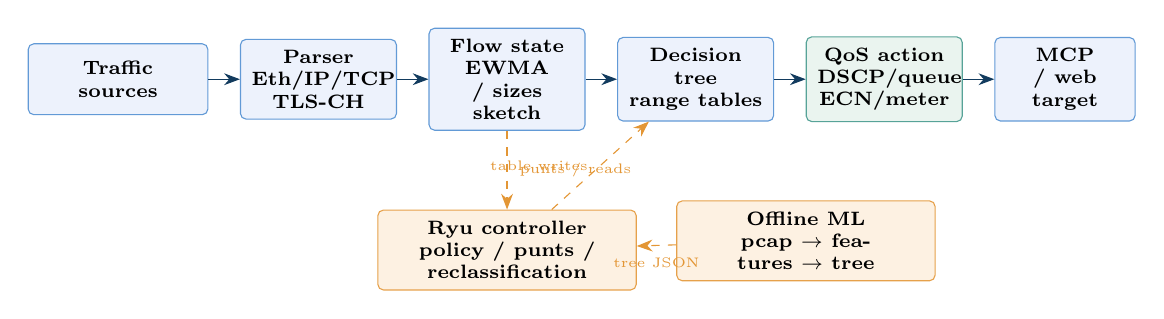
\begin{tikzpicture}[node distance=4mm, >={Stealth[length=2mm]}]
    \node[draw=deckBlue!70, fill=blockBlueBg, rounded corners=2pt, align=center,
          font=\scriptsize\bfseries, inner sep=4pt, minimum height=9mm, text width=20mm]
          (src) {Traffic\\sources};
    \node[draw=deckBlue!70, fill=blockBlueBg, rounded corners=2pt, align=center,
          font=\scriptsize\bfseries, inner sep=4pt, minimum height=9mm, text width=17mm,
          right=of src] (parse) {Parser\\Eth/IP/TCP\\TLS-CH};
    \node[draw=deckBlue!70, fill=blockBlueBg, rounded corners=2pt, align=center,
          font=\scriptsize\bfseries, inner sep=4pt, minimum height=9mm, text width=17mm,
          right=of parse] (feat) {Flow state\\EWMA / sizes\\sketch};
    \node[draw=deckBlue!70, fill=blockBlueBg, rounded corners=2pt, align=center,
          font=\scriptsize\bfseries, inner sep=4pt, minimum height=9mm, text width=17mm,
          right=of feat] (clf) {Decision tree\\range tables};
    \node[draw=deckTeal!70, fill=blockGreenBg, rounded corners=2pt, align=center,
          font=\scriptsize\bfseries, inner sep=4pt, minimum height=9mm, text width=17mm,
          right=of clf] (act) {QoS action\\DSCP/queue\\ECN/meter};
    \node[draw=deckBlue!70, fill=blockBlueBg, rounded corners=2pt, align=center,
          font=\scriptsize\bfseries, inner sep=4pt, minimum height=9mm, text width=15mm,
          right=of act] (tgt) {MCP / web\\target};

    \draw[->, deckNavy] (src) -- (parse);
    \draw[->, deckNavy] (parse) -- (feat);
    \draw[->, deckNavy] (feat) -- (clf);
    \draw[->, deckNavy] (clf) -- (act);
    \draw[->, deckNavy] (act) -- (tgt);

    \node[draw=deckAmber!80, fill=blockAmberBg, rounded corners=2pt, align=center,
          font=\scriptsize\bfseries, inner sep=4pt, minimum height=8mm, text width=30mm,
          below=10mm of feat] (ctrl) {Ryu controller\\policy / punts / reclassification};
    \node[draw=deckAmber!80, fill=blockAmberBg, rounded corners=2pt, align=center,
          font=\scriptsize\bfseries, inner sep=4pt, minimum height=8mm, text width=30mm,
          below=10mm of clf, xshift=14mm] (ml) {Offline ML\\pcap $\to$ features $\to$ tree};

    \draw[->, dashed, deckAmber!90] (feat) -- node[font=\tiny, right=1pt] {punts / reads} (ctrl);
    \draw[->, dashed, deckAmber!90] (ctrl) -- node[font=\tiny, left=1pt] {table writes} (clf);
    \draw[->, dashed, deckAmber!90] (ml) -- node[font=\tiny, below=1pt] {tree JSON} (ctrl);
  \end{tikzpicture}
  \end{center}
  \vspace{-0.2em}
  {\scriptsize \textbf{Fast path} (every packet, ns--\textmu s) stays in the switch;
  \textbf{slow path} (ms--s) only refines.}
\end{frame}

% ---------------------------------------------------------------- 7 tools
\begin{frame}{Tools Provide the Project's Technical Foundation}
  \begin{exampleblock}{What should be included?}
    Programming languages, libraries, frameworks, platforms, hardware, and datasets used to develop
    and evaluate the project.
  \end{exampleblock}
  \begin{columns}[T, onlytextwidth]
    \begin{column}{0.48\textwidth}
      \begin{itemize}
        \item \textbf{P4\textsubscript{16} (v1model)} -- data-plane language
        \item \textbf{BMv2 \texttt{simple\_switch}} -- software switch
        \item \textbf{Mininet} -- network emulation
        \item \textbf{Ryu (Python 3.9)} -- SDN controller
        \item \textbf{Python 3.11} -- tooling and ML
      \end{itemize}
    \end{column}
    \begin{column}{0.48\textwidth}
      \begin{itemize}
        \item \textbf{scikit-learn} -- decision-tree training
        \item \textbf{Scapy / tshark / tcpreplay} -- capture and replay
        \item \textbf{pandas / matplotlib} -- metrics and figures
        \item \textbf{pytest / PTF} -- Python and P4 tests
        \item \textbf{Datasets} -- agent frameworks in Docker, MAWI/CAIDA traces
      \end{itemize}
    \end{column}
  \end{columns}
\end{frame}

% ---------------------------------------------------------------- 8 modules
\begin{frame}{Modules Divide the Project into Manageable Parts}
  \begin{block}{Definition}
    Module identification divides the complete project into smaller components, each responsible
    for a specific task.
  \end{block}
  \begin{columns}[T, onlytextwidth]
    \begin{column}{0.48\textwidth}
      \begin{itemize}
        \item \textbf{Data-plane module} -- \texttt{p4src/}
        \item \textbf{Controller module} -- \texttt{controller/}
        \item \textbf{ML module} -- \texttt{ml/}
      \end{itemize}
    \end{column}
    \begin{column}{0.48\textwidth}
      \begin{itemize}
        \item \textbf{Traffic-harness module} -- \texttt{harness/}
        \item \textbf{Evaluation module} -- \texttt{eval/}
        \item \textbf{Dashboard module} -- \texttt{dashboard/}
      \end{itemize}
    \end{column}
  \end{columns}
  \vspace{0.4em}
  \begin{alertblock}{Shared contract layer}
    All six modules import names, class labels, DSCP/queue maps, feature order, and schemas from
    \textbf{\texttt{common/contracts.py}} --- the single frozen source of truth. No module
    re-declares a literal.
  \end{alertblock}
\end{frame}

% ---------------------------------------------------------------- 9 module I/P/O
\begin{frame}{Explain Every Module Through Input, Process, and Output}
  \begin{block}{Module explanation}
    Describe the purpose, input, processing steps, and output of every identified module.
  \end{block}
  \vspace{-0.2em}
  {\scriptsize
  \begin{center}
  \begin{tabular}{@{}p{2.1cm}p{3.1cm}p{3.4cm}p{3.2cm}@{}}
    \toprule
    \textbf{Module} & \textbf{Input} & \textbf{Process} & \textbf{Output}\\
    \midrule
    Data plane & Packets on the choke link & Parse, update flow registers, tree lookup, QoS action
      & Forwarded packet + DSCP/queue/ECN\\
    Controller & Punted first packets, register reads & JA4, Web Bot Auth, reclassification sweep
      & Table/policy writes, overrides\\
    ML & Labelled pcaps & Feature extraction, tree training (depth $\leq$ 8), compile to entries
      & Tree JSON $\to$ table entries\\
    Harness & Agent frameworks, trace replay & Run scenarios, capture, join labels to 5-tuples
      & \texttt{labels.csv}, pcaps\\
    Evaluation & Experiment YAML + seed & Run grid over 4 baselines, extract percentiles
      & Metrics, CIs, figures\\
    Dashboard & Live per-class counters & Aggregate p50/p95/p99 & Demo view\\
    \bottomrule
  \end{tabular}
  \end{center}}
  \vspace{0.1em}
  \begin{alertblock}{Example: Harness labelling module (implemented for Review 1)}
    \footnotesize \textbf{Input:} pcap + orchestration windows ·
    \textbf{Process:} extract TCP/UDP 5-tuples, join to windows deterministically ·
    \textbf{Output:} frozen-schema \texttt{labels.csv}
  \end{alertblock}
\end{frame}

% ---------------------------------------------------------------- 10 algorithm
\begin{frame}{Choose an Algorithm and Explain How It Works}
  \begin{columns}[T, onlytextwidth]
    \begin{column}{0.48\textwidth}
      \begin{block}{Algorithm identification}
        \small \textbf{Decision tree (depth $\leq$ 8)}, trained offline in scikit-learn and
        mechanically compiled into P4 \textbf{range-match tables}.
      \end{block}
    \end{column}
    \begin{column}{0.48\textwidth}
      \begin{exampleblock}{Why this algorithm}
        \small A tree is the one model a switch can evaluate in a fixed number of table lookups ---
        no loops, no floating point, bounded per-packet cost.
      \end{exampleblock}
    \end{column}
  \end{columns}
  \begin{alertblock}{How it works}
    \small
    Ten integer features (timing EWMA, packet sizes, byte ratios, fan-out sketch) are computed in
    registers with \textbf{saturating fixed-point} arithmetic --- shifts only, no division.
    Each tree path becomes one table entry over feature ranges; the matched entry yields a 2-bit
    class, which directly selects the QoS action. Classification is re-evaluated at packet
    checkpoints \textbf{6, 16, and 64}; before the first checkpoint the flow is UNKNOWN and served
    best-effort.
  \end{alertblock}
  \vspace{-0.2em}
  {\scriptsize \textbf{Review 1 status:} the label-join path is implemented; bit-exact feature
  arithmetic is \emph{explicitly blocked} pending four frozen-contract decisions
  (\texttt{docs/feature\_arithmetic\_design\_gaps.md}).}
\end{frame}

% ---------------------------------------------------------------- 11 first 25%
\begin{frame}{The First 25\% Should Demonstrate Visible Progress}
  \begin{exampleblock}{Expected milestone}
    Approximately one-fourth of the planned development work completed and supported by initial
    evidence or a working prototype.
  \end{exampleblock}
  \vspace{-0.2em}
  {\footnotesize
  \begin{itemize}
    \item \textbf{Contracts frozen and tested} -- class treatments, table/register names, feature
          order, CPU header, label and tree schemas in \texttt{common/contracts.py}.
    \item \textbf{M1 forwarding prototype} -- \texttt{p4src/l2fwd.p4} with the L2 table and a
          readable \texttt{policy\_version} register.
    \item \textbf{Topology} -- deterministic \texttt{choke\_v1} host, port, and bottleneck
          definition.
    \item \textbf{Controller read path} -- BMv2 CLI boundary with validated register reads and
          explicit error reporting.
    \item \textbf{Initial preprocessing} -- orchestration-to-\texttt{labels.csv} pcap labelling in
          the frozen schema.
    \item \textbf{Reproducibility} -- seeded Review 1 smoke config; \texttt{make review-1-host}
          runs the whole host gate.
  \end{itemize}}
  \vspace{-0.1em}
  \begin{block}{Verified vs pending}
    \footnotesize
    \textbf{Passing on host:} Ruff lint + format, \textbf{34 pytest tests}, config validation,
    \texttt{AGENTS.md}/\texttt{CLAUDE.md} byte-identical. \\
    \textbf{Awaiting the Linux VM:} live Mininet/BMv2 run and one iperf3 flow across the switch. \\
    \textbf{Not claimed yet:} no classification-accuracy, p99-reduction, or overhead result.
  \end{block}
\end{frame}

\end{document}
